\newpage
\section{Sprint 3}

Siguiendo la planificación inicial, el tercer sprint se centra en la implementación del procesado multimedia en el servidor (generación de miniaturas, compresión de imágenes y vídeos, etiquetado basado en metadatos, etc.) y en el cliente móvil la subida de archivos multimedia al servidor y la visualización de los archivos subidos.

El objetivo es entregar un incremento funcional que permita al usuario subir fotos y vídeos desde el móvil, que el servidor procese estos archivos (compresión, miniaturas) y que puedan visualizarse en una galería online básica. Se priorizan historias que permitan una experiencia de usuario completa de subida y visualización, así como la robustez y eficiencia del proceso.

\subsection{Historias de usuario}
A continuación se presentan las historias de usuario y técnicas seleccionadas para este sprint, siguiendo el mismo formato que en los sprints anteriores. El desglose en tareas se realizará posteriormente.

Las historias seleccionadas son las siguientes:
\begin{itemize}
    % Servidor (prioridad máxima)
    \item HU01: Subida de fotos -- 5 PH
    \item HU04: Subida de vídeos -- 5 PH
    \item HT09: Compresión de imágenes -- 5 PH
    \item HT10: Subida concurrente -- 8 PH
    \item HU09: Galería visual -- 5 PH
    \item HT17: Notificaciones de progreso -- 3 PH
    % Cliente móvil (imprescindible para probar subida y visualización)
    \item HU16: Seleccionar fotos -- 3 PH
    \item HU27: Subir vídeos -- 5 PH
    \item HU18: Ver progreso de subida -- 8 PH
\end{itemize}

La suma total de las historias seleccionadas es de \textbf{47 puntos de historia (PH)}. Esta selección se ha ajustado para priorizar el procesado multimedia en el servidor y solo las funcionalidades imprescindibles del cliente móvil, manteniendo una carga realista y coherente con la capacidad demostrada en los sprints anteriores (34–56 PH). Se han dejado fuera historias menos críticas para el objetivo de este sprint, como la cancelación de subida, sincronización manual, galería online avanzada, manejo de errores de red y estadísticas de copia, que se abordarán en sprints posteriores.

La descomposición en tareas de desarrollo de las historias de usuario se pueden encontrar en el apéndice \ref{appendix:sprint3-backlog}.

El total de horas estimadas para las tareas de desarrollo del Sprint 3 es de \textbf{46 horas}, cifra que se aproxima a la capacidad teórica del sprint. La distribución es la siguiente:

\begin{itemize}
    \item HU01 (Subida de fotos): 6 horas
    \item HU04 (Subida de vídeos): 6 horas
    \item HT09 (Compresión de imágenes): 5 horas
    \item HT10 (Subida concurrente): 7.5 horas
    \item HU09 (Galería visual): 5 horas
    \item HT17 (Notificaciones de progreso): 2.5 horas
    \item HU16 (Seleccionar fotos móvil): 3 horas
    \item HU27 (Subir vídeos móvil): 4.5 horas
    \item HU18 (Ver progreso de subida móvil): 6.5 horas
\end{itemize}

\subsection{Diagrama de Gantt}
Una vez definidas las tareas para cada historia de usuario, se ha elaborado un diagrama de Gantt para visualizar la planificación del sprint. Este diagrama muestra el orden de las tareas y su duración estimada:

\begin{figure}[H]
    \begin{center}
        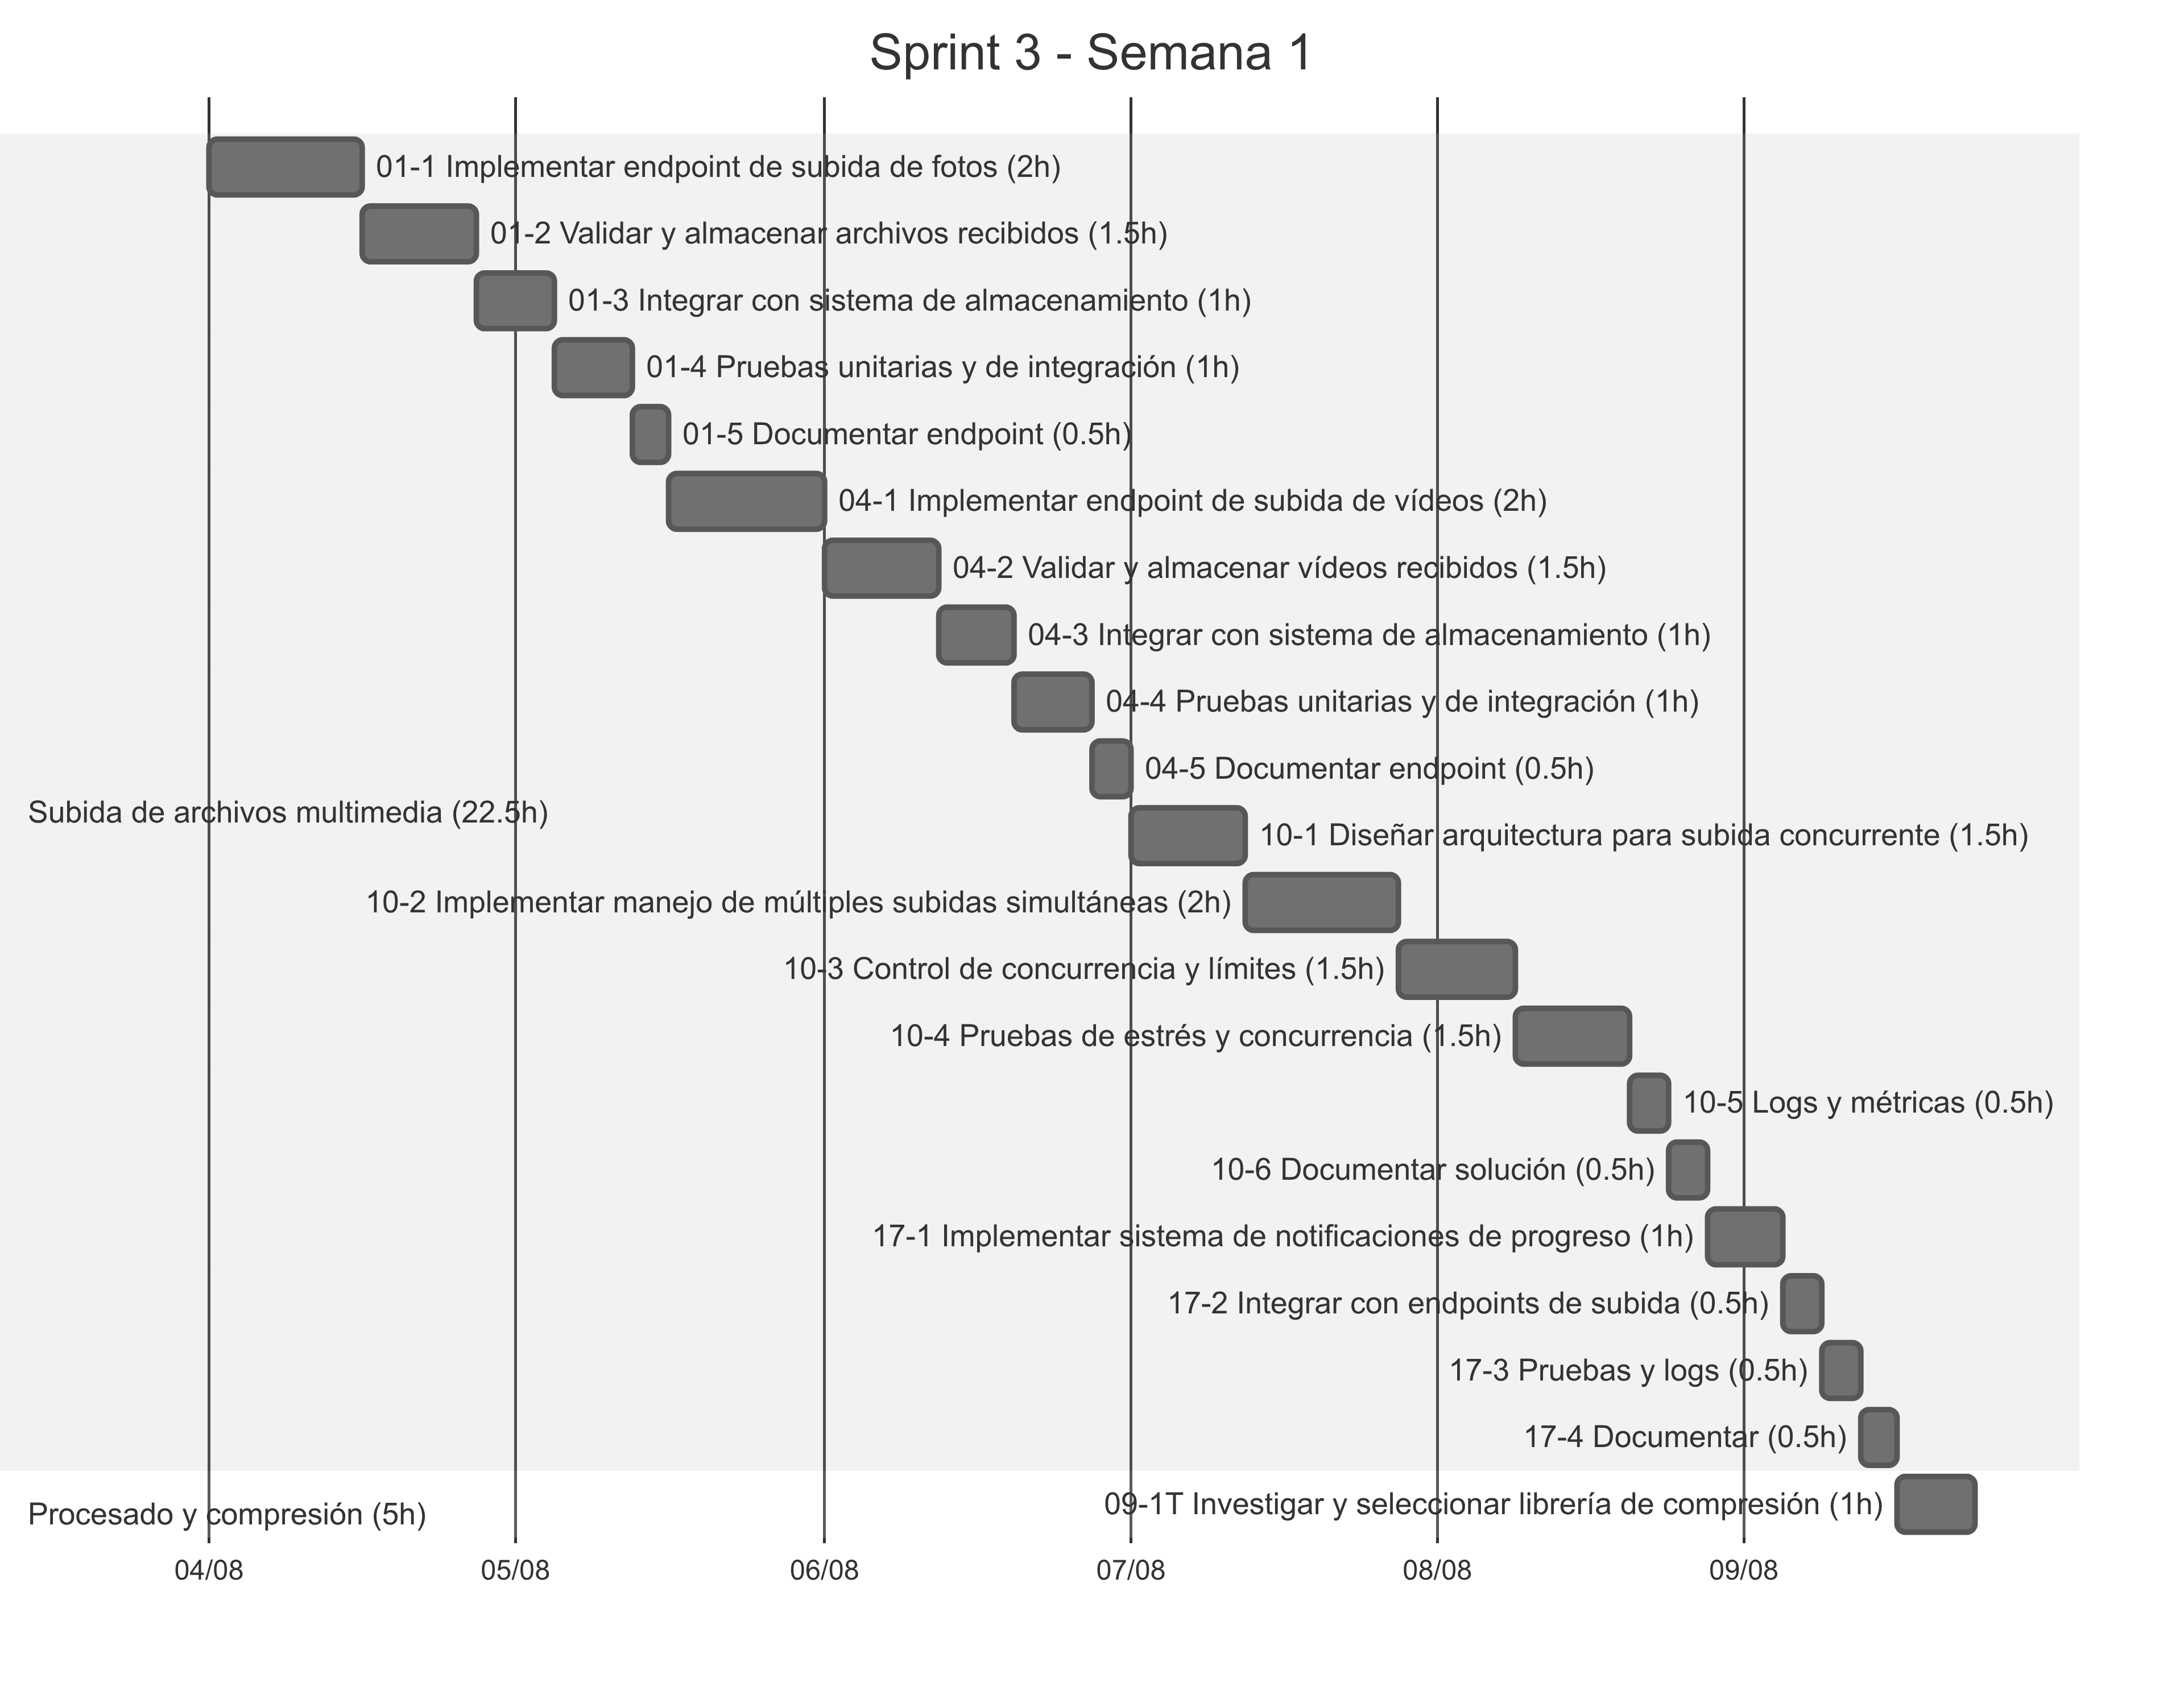
\includegraphics[width=0.8\textwidth]{assets/sprint3/week1-gantt.png}
    \end{center}
    \caption{Diagrama de Gantt de las tareas de la primera semana del sprint 3}\label{fig:gantt-sprint3-week1}
\end{figure}


\begin{figure}[H]
    \begin{center}
        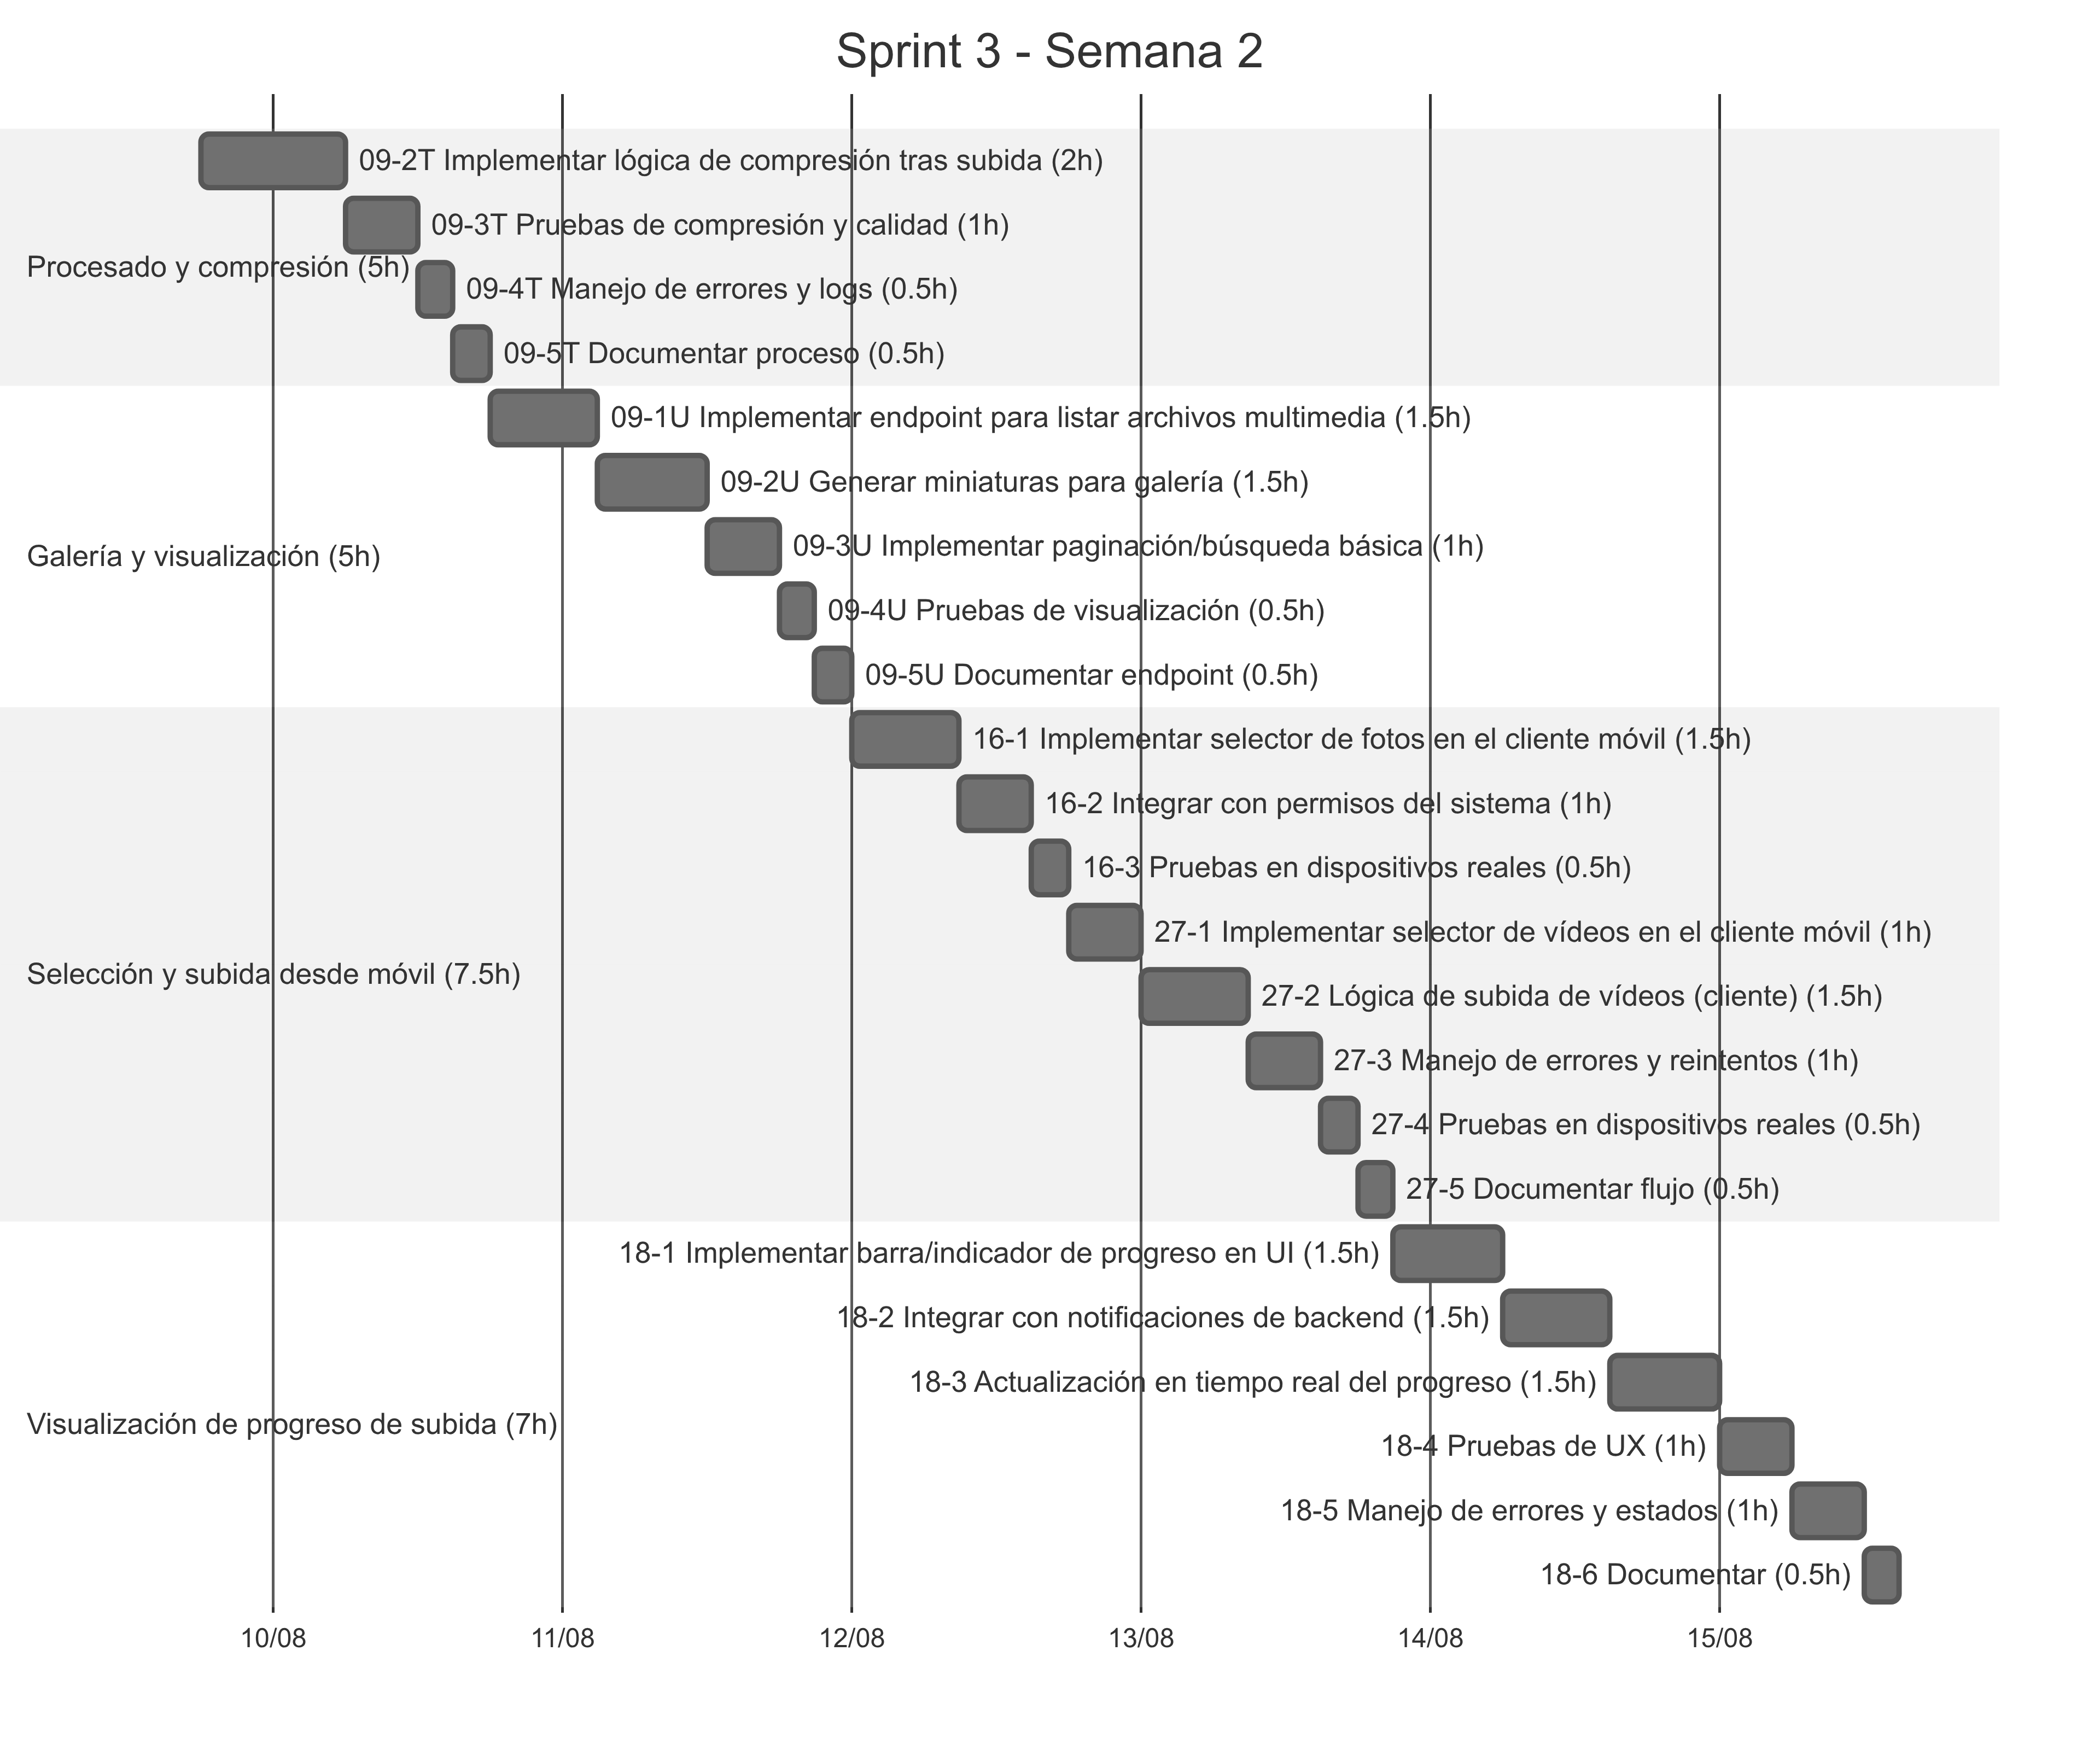
\includegraphics[width=0.8\textwidth]{assets/sprint3/week2-gantt.png}
    \end{center}
    \caption{Diagrama de Gantt de las tareas de la segunda semana del sprint 3}\label{fig:gantt-sprint3-week2}
\end{figure}

En este sprint se han priorizado las tareas relacionadas principalmente con el procesado multimedia en el servidor, dado que en el anterior sprint el enfoque estuvo en el desarrollo de la aplicación móvil.

Las tareas relacionadas con la aplicación móvil de este sprint se centran principalmente en integrar los cambios implementados en el servidor.
Se realiza de esta manera para que al finalizar el sprint 3 tengamos un producto con más valor, puesto que el usuario tendrá la posibilidad de subir fotos y vídeos desde su móvil, que serán procesados en el servidor y podrán visualizarse en una galería online.

\subsection{Diseño detallado e implementación}
\subsubsection{Modelo Entidad-Relación}

Para este sprint se han realizado cambios en el modelo entidad-relación para soportar las nuevas funcionalidades de subida y gestión de archivos multimedia.
El modelo de entidad-relación actualizado sería el siguiente:

\begin{figure}[H]
    \begin{center}
        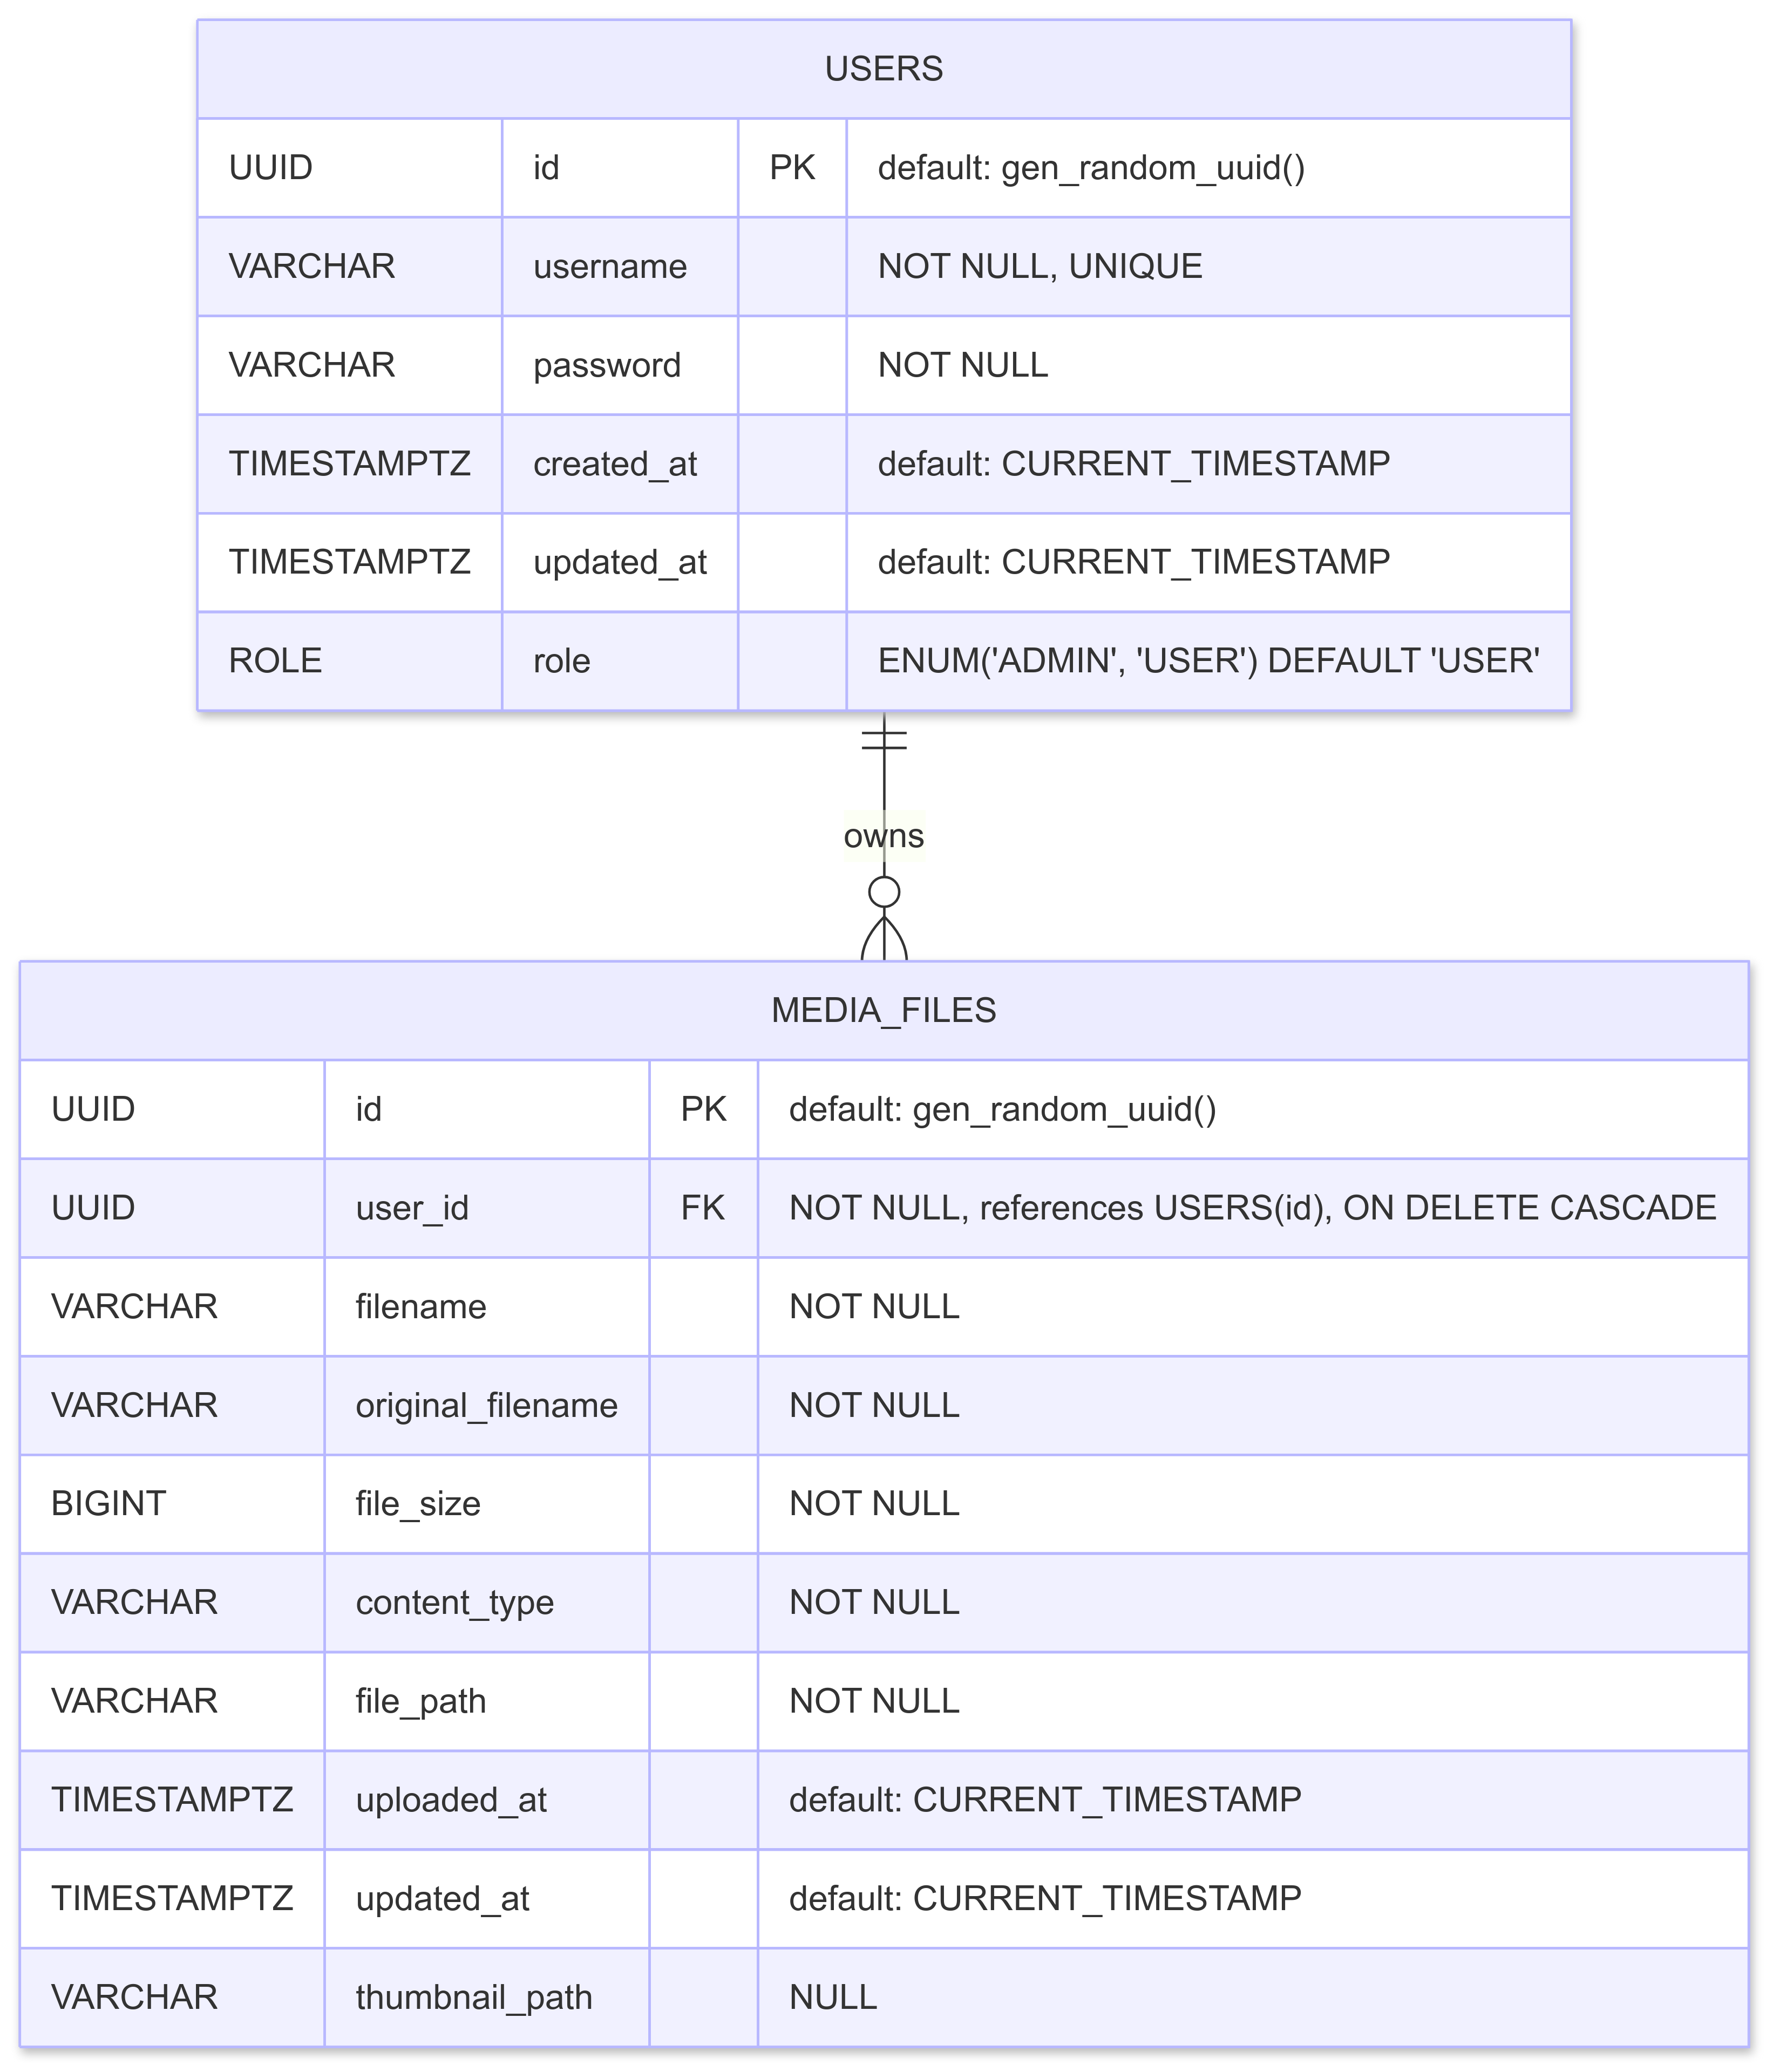
\includegraphics[width=0.8\textwidth]{assets/sprint3/media-files-er-diagram.png}
    \end{center}
    \caption{Diagrama Entidad-Relación actualizado con la entidad MediaFile}\label{fig:media-files-er-diagram}
\end{figure}

Como se puede ver en la figura, la entidad usuarios se ha mantenido igual y se ha añadido una nueva entidad llamada MEDIA\_FILES, que representa los metadatos de los archivos multimedia subidos por los usuarios.


\subsubsection{Subida de archivos multimedia}

Se ha realizado la implementación de la subida de archivos multimedia (fotos y vídeos) desde la aplicación móvil al servidor, así como el procesado de estos archivos en el servidor (compresión de imágenes, generación de miniaturas) y la visualización en una galería online.

El flujo que se ha seguido en la implementación de la subida de los archivos multimedia ha sido el siguiente:
\begin{figure}[H]
    \begin{center}
        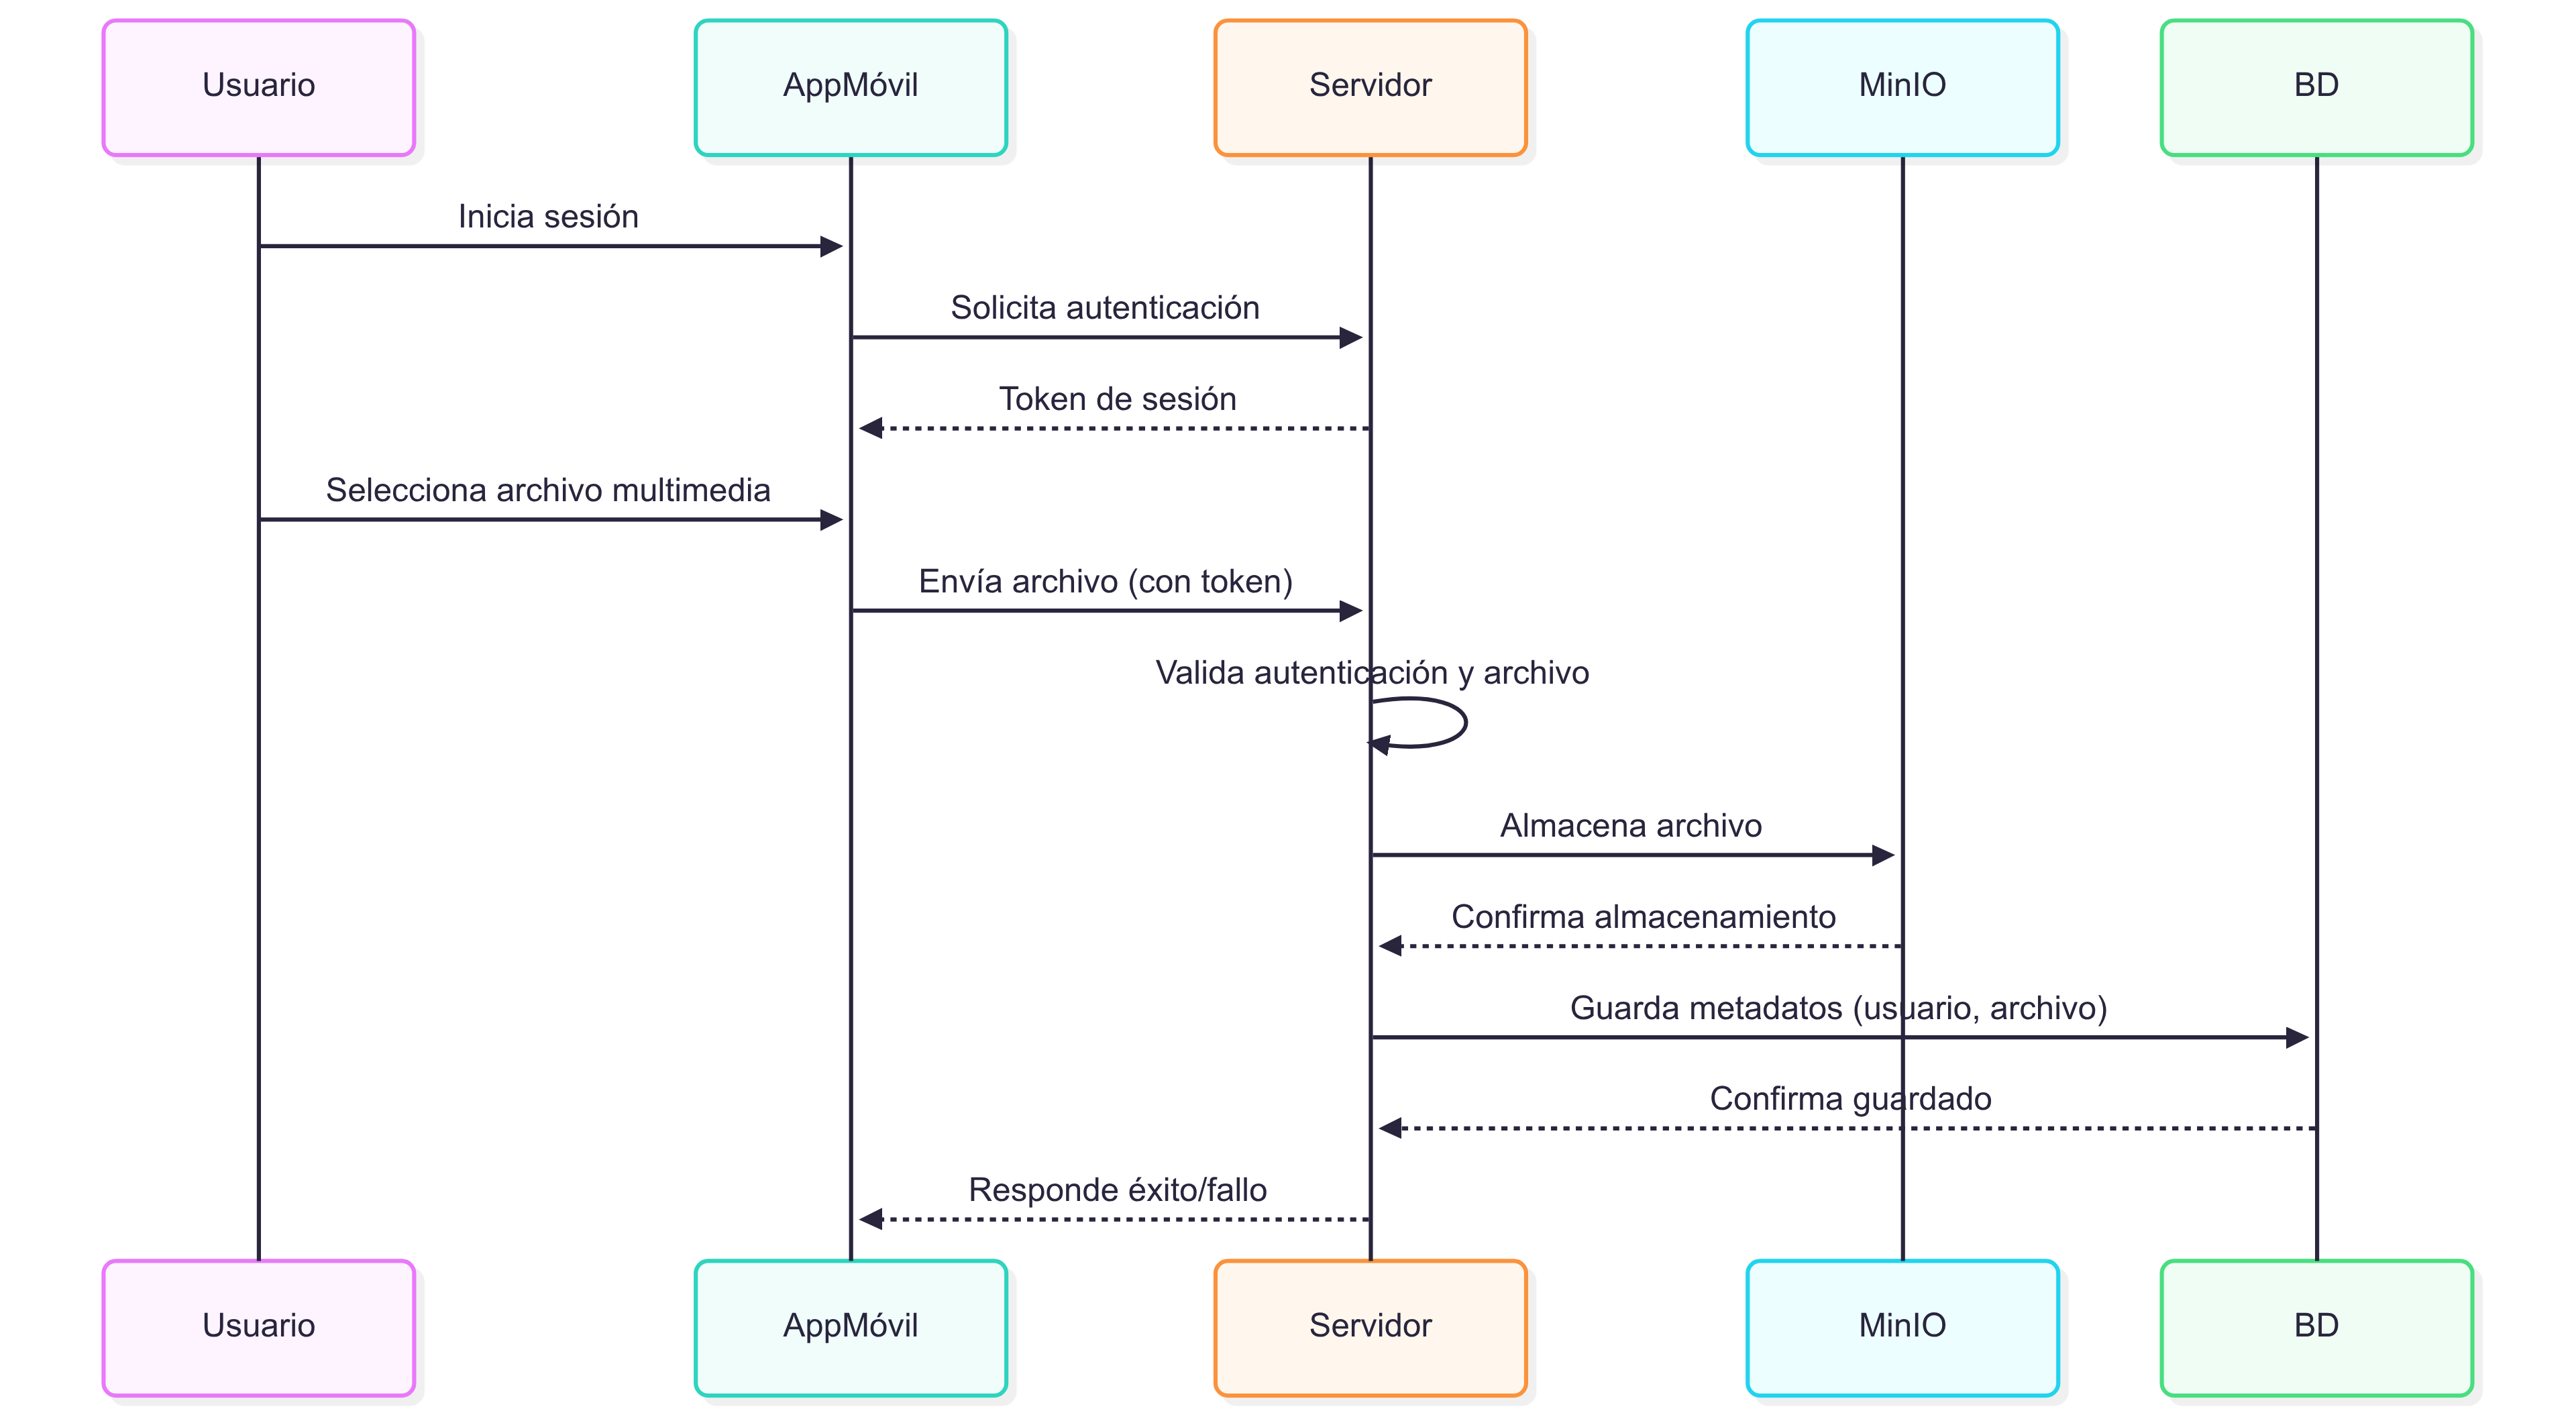
\includegraphics[width=0.95\textwidth]{assets/sprint3/diagrama-subida-archivos.png}
    \end{center}
    \caption{Diagrama de flujo de subida de un archivo multimedia}\label{fig:diagrama-flujo-subida-archivos}
\end{figure}

Como se muestra en la Figura \ref{fig:diagrama-flujo-subida-archivos}, el usuario selecciona la foto o video que desea subir desde la aplicación móvil. La aplicación móvil envía los archivos al servidor a través de un endpoint de subida. El servidor recibe el archivo y lo procesa sin alojar todo el contenido del mismo en memoria, consiguiendo así un procesamiento eficiente. A continuación, el servidor procesa el archivo y genera una miniatura. Finalmente, los archivos procesados se almacenan en el sistema de almacenamiento definitivo (MinIO) y el usuario puede ver sus archivos en una galería online, es decir, no necesita tener los archivos en su dispositivo para poder visualizarlos.

La generación de miniaturas se realiza de manera paralela, por lo que no bloquea la subida de archivos.

\subsubsection{Manejo de subidas concurrentes}

Durante el desarrollo se realizaron varias pruebas de estrés de subida de diferentes números de archivos (100, 1000, 20000) para asegurar que el servidor podía manejar múltiples subidas concurrentes sin errores ni bloqueos. Se implementó un sistema de control de concurrencia para limitar el número de subidas simultáneas, evitando así la sobrecarga del servidor.
Para la gestión de subidas concurrentes se ha definido un número máximo de peticiones que pueden ser atendidas de forma simultánea. Este ajuste es configurable a través de una variable de entorno, permitiendo así adaptar el comportamiento del servidor según la capacidad del entorno de despliegue.

El principal problema que se encontró durante las pruebas de estrés fue la saturación de la memoria del servidor al recibir demasiadas peticiones simultáneas de subida de archivos. Para cada archivo que se quería subir se tenía que alojar una cantidad de memoria, bloqueando el servidor para muchas peticiones concurrentes. Aunque el servidor manejara los archivos de manera eficiente, es decir, sin cargar todo el archivo en memoria, tener 200 peticiones en paralelo cada una alojando 8MB se traduce en 1.6GB (sin tener en cuenta el overhead que se produce al crear un thread para cada petición). Para solucionar este problema, se implementó un sistema de semáforos que gestiona las peticiones entrantes y establece un límite de peticiones que pueden ejecutarse en paralelo, asegurando así que el servidor no se sobrecargue.

\subsubsection{Estado de subida de los archivos multimedia}
En la aplicación móvil se ha implementado una galería que muestra los archivos multimedia locales junto con su estado, de esta manera el usuario sabe qué archivos de su dispositivo ya han sido subidos al servidor y cuáles están pendientes de subir.
Para ello, no ha sido necesario almacenar el estado de los archivos en una base de datos local, sino que se han utilizado las propiedades de los archivos locales que nos ofrecen los dispositivos. A la hora de subir un archivo, este se sube con un nombre de archivo único que hace referencia a el id del archivo en el dispositivo local. De esta manera, al listar los archivos locales, se puede comprobar, mediante la lista de archivos subidos consultada del servidor, si el archivo ya ha sido subido o no.

Gracias a esta solución, cada archivo en el servidor es único, evitando así subidas duplicadas y manteniendo la integridad de los datos.

\subsection{Extensión del sprint y retos técnicos}

Durante el desarrollo del Sprint 3 se encontraron dificultades técnicas significativas que requirieron una semana adicional para completar las funcionalidades planificadas. Los principales retos surgieron por las limitaciones de la tecnología LynxJS utilizada en el desarrollo de la aplicación móvil, especialmente en el manejo de subidas de archivos.

\subsubsection{Limitaciones críticas de LynxJS}

La principal limitación técnica encontrada fue la **ausencia de soporte nativo para subidas multipart** en LynxJS. Esta carencia impactó severamente en las siguientes áreas:

\begin{itemize}
    \item \textbf{Subidas multipart nativas}: LynxJS no proporciona APIs para manejar subidas de archivos multipart, obligando a implementar toda la funcionalidad de transferencia de archivos desde cero utilizando módulos nativos del sistema operativo.
    
    \item \textbf{Tracking de progreso de subida}: La falta de soporte multipart imposibilita el seguimiento granular del progreso de subida, ya que las implementaciones nativas requeridas no exponen interfaces compatibles con el sistema de eventos de LynxJS.
    
    \item \textbf{Gestión de archivos grandes}: El manejo de vídeos y archivos multimedia de gran tamaño requiere implementaciones nativas complejas que van más allá del scope actual del framework.
\end{itemize}

\subsubsection{Historia de usuario no completada}

Debido a estas limitaciones técnicas, la historia HU18 (Ver progreso de subida) no pudo ser completada en este sprint. Los motivos específicos son:

\begin{itemize}
    \item La implementación nativa de subidas multipart consume todo el tiempo estimado sin permitir la integración del sistema de progreso.
    \item El desarrollo de un puente de comunicación entre los módulos nativos y LynxJS para el tracking de progreso requiere un análisis arquitectónico más profundo.
    \item Las pruebas de integración entre componentes nativos y el framework presentan complejidades adicionales no contempladas inicialmente.
\end{itemize}

Esta funcionalidad se ha pospuesto para el Sprint 4, donde se dedicará tiempo específico a desarrollar una arquitectura robusta que permita la comunicación bidireccional entre módulos nativos y LynxJS.

\subsubsection{Impacto en el cronograma}

El tiempo adicional de una semana se destinó a:
\begin{enumerate}
    \item Investigación de limitaciones de LynxJS para subidas multipart (8 horas)
    \item Implementación completa de módulos nativos para subida de archivos (16 horas)
    \item Refactorización de HU16 y HU27 para usar implementaciones nativas (12 horas)
    \item Pruebas de integración y compatibilidad (8 horas)
\end{enumerate}

A pesar de la extensión, se ha logrado entregar un incremento funcional que permite la subida de fotos y vídeos, cumpliendo con los objetivos principales del sprint. La funcionalidad de progreso de subida se abordará en el siguiente sprint con una planificación específica para superar las limitaciones arquitectónicas identificadas.

\subsubsection{Historia de usuario parcialmente completada}

La historia de usuario HU27, correspondiente a la subida de vídeos desde el cliente móvil, no se ha podido completar en su totalidad. Aunque la funcionalidad de subida está implementada, la visualización de los vídeos en la aplicación no ha sido posible debido a la complejidad de la implementación del componente de vídeo nativo. Esta tarea ha consumido más tiempo del estimado inicialmente, y se ha decidido posponer la funcionalidad de visualización para un futuro sprint para no comprometer la entrega de otras funcionalidades.
